\documentclass[12pt]{report}
\usepackage[utf8]{inputenc}
\setlength{\textwidth}{14cm}
\setlength{\parindent}{0em}
\setlength{\parskip}{1em}
\usepackage[T1]{fontenc}

%für text neben bild
\usepackage{float}
\usepackage{graphicx}

\usepackage{pgfplots}
\DeclareUnicodeCharacter{2212}{−}
\usepgfplotslibrary{groupplots,dateplot}
\usetikzlibrary{patterns,shapes.arrows}
\pgfplotsset{compat=newest}

\usepackage{graphicx}
\graphicspath{{images/}}
\usepackage[a4paper, width=150mm, top=30mm, bottom=30mm]{geometry}

\usepackage{booktabs}

\usepackage{fancyhdr}
\pagestyle{fancy}
\renewcommand{\chaptermark}[1]{\markboth{#1}{}}\tabularnewline
\setlength{\headheight}{15pt}
\fancypagestyle{plain}{}{
	\fancyhead{}
	\fancyhead[L]{Thesis Title}
	\fancyhead[R]{\leftmark}
	\fancyfoot{}
	\fancyfoot[R]{\thepage}
	\fancyfoot[L]{Simon Gutwein}
}

\usepackage{caption}
\usepackage{subcaption}
\usepackage{enumitem}
\usepackage[colorlinks=false]{hyperref}

\usepackage{titlesec}
\titleformat{\chapter}[display]{\normalfont\bfseries}{}{0pt}{\Huge}
\titleformat{\section}[display]{\normalfont\bfseries}{}{0pt}{\Large}
\titlespacing*{\chapter}{0pt}{-20pt}{20pt}
\titlespacing*{\section}{0pt}{10pt}{20pt}

\title{
	\centering
	%{\scshape\LARGE Eberhard-Karls Universität \\ Tübingen \par}
	%\vspace{1cm}
	
\includegraphics[width=0.5\textwidth]{logo4}\par\vspace{1cm}
	
\includegraphics[width=0.15\textwidth]{logo3}\par\vspace{1cm}
	{\huge\bfseries Fast Dose Estimation for Radiotherapy Treatment Plans with Uncertainty Estimation\par}
	\vspace{1cm}
	{\fontsize{20.74}{0}\selectfont Master Thesis}\vspace{3cm}
	\vfill
	{\fontsize{17}{18}\selectfont supervised by \fontsize{17}{18}\selectfont\\ Prof. Dr. Daniela Thorwarth and Dr. Christian Baumgartner}
	\vfill
}


\usepackage{titling}
\setlength{\droptitle}{-2cm}

\author{Simon Gutwein}
\date{\today}

\renewcommand{\headrulewidth}{0.4pt}
\renewcommand{\footrulewidth}{0.4pt}

\usepackage[sorting=none]{biblatex}
\addbibresource{/Users/simongutwein/Documents/GitHub/Master_Thesis/Masterarbeit_Text/BibTex/Masterarbeit.bib}

\begin{document}

\maketitle

\chapter{Aufbau}
\section{BlaBla}

Lorem ipsum dolor sit amet, consetetur sadipscing elitr, sed diam nonumy eirmod tempor invidunt ut labore et dolore magna aliquyam erat, sed diam voluptua. At vero eos et accusam et justo duo dolores et ea rebum. Stet clita kasd gubergren, no sea takimata sanctus est Lorem ipsum dolor sit amet. Lorem ipsum dolor sit amet, consetetur sadipscing elitr, sed diam nonumy eirmod tempor invidunt ut labore et dolore magna aliquyam erat, sed diam voluptua. At vero eos et accusam et justo duo dolores et ea rebum. Stet clita kasd gubergren, no sea takimata sanctus est Lorem ipsum dolor sit amet.

\begin{center}
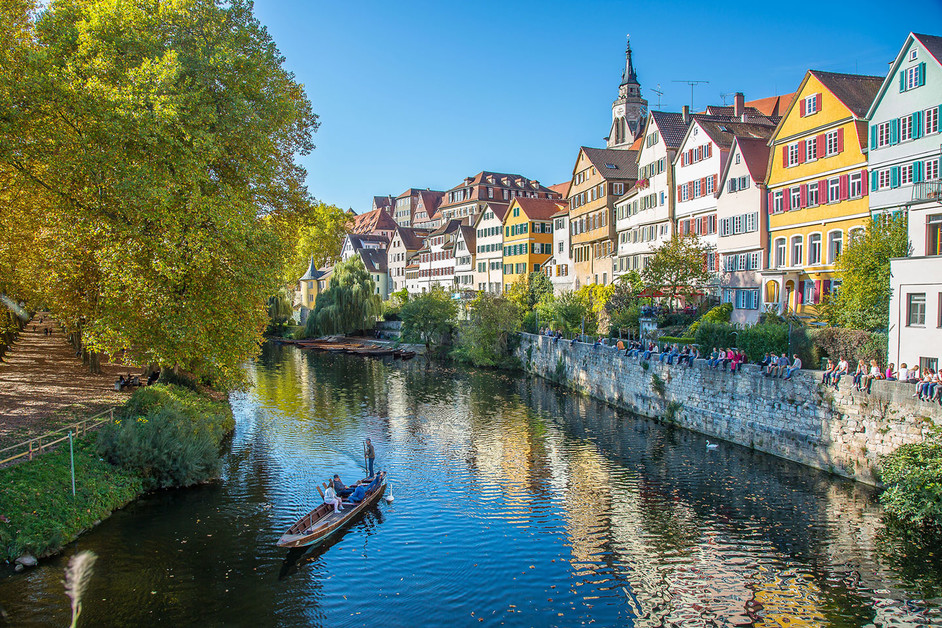
\includegraphics[width=300pt]{Neckarfront.jpg}
\end{center}

\section{BlaBla}
Lorem ipsum dolor sit amet, consetetur sadipscing elitr, sed diam nonumy eirmod tempor invidunt ut labore et dolore magna aliquyam erat, sed diam voluptua. At vero eos et accusam et justo duo dolores et ea rebum. Stet clita kasd gubergren, no sea takimata sanctus est Lorem ipsum dolor sit amet. Lorem ipsum dolor sit amet, consetetur sadipscing elitr, sed diam nonumy eirmod tempor invidunt ut labore et dolore magna aliquyam erat, sed diam voluptua. At vero eos et accusam et justo duo dolores et ea rebum. Stet clita kasd gubergren, no sea takimata sanctus est Lorem ipsum dolor sit amet.

% \chapter{Fake Abstract}
% \section{BlaBla}

Lorem ipsum dolor sit amet, consetetur sadipscing elitr, sed diam nonumy eirmod tempor invidunt ut labore et dolore magna aliquyam erat, sed diam voluptua. At vero eos et accusam et justo duo dolores et ea rebum. Stet clita kasd gubergren, no sea takimata sanctus est Lorem ipsum dolor sit amet. Lorem ipsum dolor sit amet, consetetur sadipscing elitr, sed diam nonumy eirmod tempor invidunt ut labore et dolore magna aliquyam erat, sed diam voluptua. At vero eos et accusam et justo duo dolores et ea rebum. Stet clita kasd gubergren, no sea takimata sanctus est Lorem ipsum dolor sit amet. Siehe \ref{fig:Neckarfront}

\begin{figure}
\center
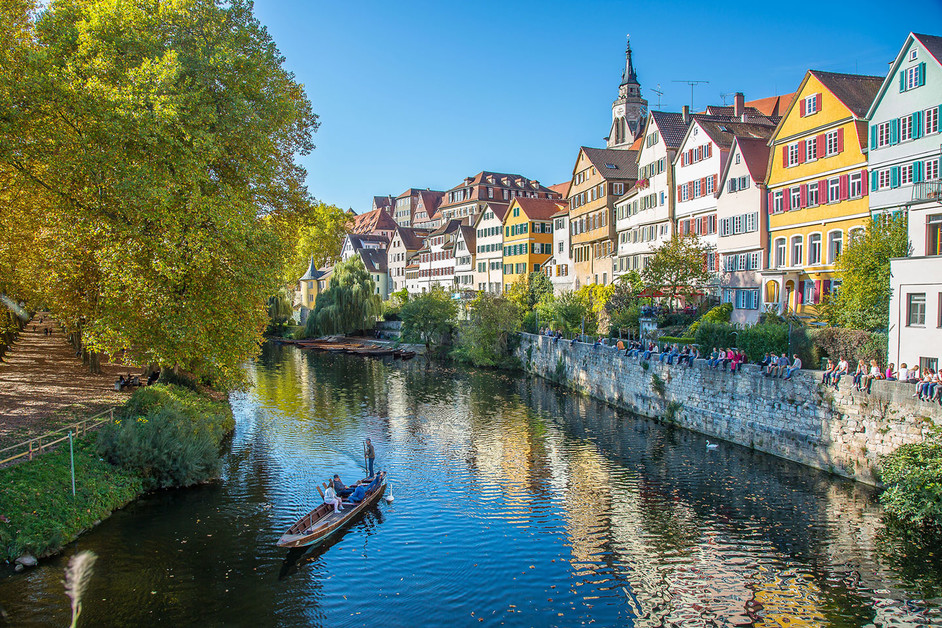
\includegraphics[width=300pt]{Neckarfront.jpg}
\caption{Neckarfront}
\label{fig:Neckarfront}
\end{figure}

\section{BlaBla}
Lorem ipsum dolor sit amet, consetetur sadipscing elitr, sed diam nonumy eirmod tempor invidunt ut labore et dolore magna aliquyam erat, sed diam voluptua. At vero eos et accusam et justo duo dolores et ea rebum. Stet clita kasd gubergren, no sea takimata sanctus est Lorem ipsum dolor sit amet. Lorem ipsum dolor sit amet, consetetur sadipscing elitr, sed diam nonumy eirmod tempor invidunt ut labore et dolore magna aliquyam erat, sed diam voluptua. At vero eos et accusam et justo duo dolores et ea rebum. Stet clita kasd gubergren, no sea takimata sanctus est Lorem ipsum dolor sit amet.\cite{thorwarth_technical_2021}
Lorem ipsum dolor sit amet, consetetur sadipscing elitr, sed diam nonumy eirmod tempor invidunt ut labore et dolore magna aliquyam erat, sed diam voluptua. At vero eos et accusam et justo duo dolores et ea rebum. Stet clita kasd gubergren, no sea takimata sanctus est Lorem ipsum dolor sit amet. Lorem ipsum dolor sit amet,\cite{davis_glioblastoma_2016, neph_deepmc_2021} consetetur sadipscing elitr, sed diam nonumy eirmod tempor invidunt ut labore et dolore magna aliquyam erat, sed diam voluptua. At vero eos et accusam et justo duo dolores et ea rebum. Stet clita kasd gubergren, no sea takimata sanctus est Lorem ipsum dolor sit amet.Lorem ipsum dolor sit amet, consetetur sadipscing elitr, sed diam nonumy eirmod tempor invidunt ut labore et dolore magna aliquyam erat, sed diam voluptua. At vero eos et accusam et justo duo dolores et ea rebum. Stet clita kasd gubergren, no sea takimata sanctus est Lorem ipsum dolor sit amet. Lorem ipsum dolor sit amet, consetetur sadipscing elitr, sed diam nonumy eirmod tempor invidunt ut labore et dolore magna aliquyam erat, sed diam voluptua. At vero eos et accusam et justo duo dolores et ea rebum. Stet clita kasd gubergren, no sea takimata sanctus est Lorem ipsum dolor sit amet.Lorem ipsum dolor sit amet, consetetur sadipscing elitr, sed diam nonumy eirmod tempor invidunt ut labore et dolore magna aliquyam erat, sed diam voluptua. At vero eos et accusam et justo duo dolores et ea rebum. Stet clita kasd gubergren, no sea takimata sanctus est Lorem ipsum dolor sit amet. Lorem ipsum dolor sit amet, consetetur sadipscing elitr, sed diam nonumy eirmod tempor invidunt ut labore et dolore magna aliquyam erat, sed diam voluptua. At vero eos et accusam et justo duo dolores et ea rebum. Stet clita kasd gubergren, no sea takimata sanctus est Lorem ipsum dolor sit amet.Lorem ipsum dolor sit amet, consetetur sadipscing elitr, sed diam nonumy eirmod tempor invidunt ut labore et dolore magna aliquyam erat, sed diam voluptua. At vero eos et accusam et justo duo dolores et ea rebum. Stet clita kasd gubergren, no sea takimata sanctus est Lorem ipsum dolor sit amet. Lorem ipsum dolor sit amet, consetetur sadipscing elitr, sed diam nonumy eirmod tempor invidunt 


\begin{figure}
	\centering
	\begin{subfigure}[b]{0.45\textwidth}
		\centering
		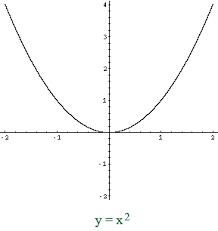
\includegraphics[width=\textwidth,height=60mm]{x_squared}
		\caption{$y = x^2$}
		\label{fig: x_squared}
	\end{subfigure}
	\hfill
	\begin{subfigure}[b]{0.45\textwidth}
		\centering
		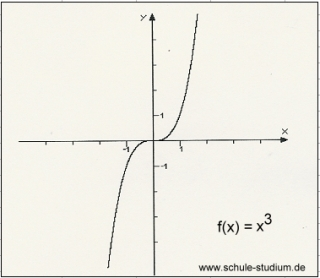
\includegraphics[width=\textwidth,height=60mm]{x_cubed}
		\caption{$y = x^3$}
		\label{fig: x_cubed}
	\end{subfigure}
	\caption{2 Simple Functions}
	\label{fig: 2 func}
\end{figure}


ut labore et dolore magna aliquyam erat, sed diam voluptua. At vero eos et accusam et justo duo dolores et ea rebum. Stet clita kasd gubergren, no sea takimata sanctus est Lorem ipsum dolor sit amet.Lorem ipsum dolor sit amet, consetetur sadipscing elitr, sed diam nonumy eirmod tempor invidunt ut labore et dolore magna aliquyam erat, sed diam voluptua. At vero eos et accusam et justo duo dolores et ea rebum. Stet clita kasd gubergren, no sea takimata sanctus est Lorem ipsum dolor sit amet. Lorem ipsum dolor sit amet, consetetur sadipscing elitr, sed diam nonumy eirmod tempor invidunt ut labore et dolore magna aliquyam erat, sed diam voluptua. At vero eos et accusam et justo duo dolores et ea rebum. Stet clita kasd gubergren, no sea takimata sanctus est Lorem ipsum dolor sit amet.Lorem ipsum dolor sit amet, consetetur sadipscing elitr, sed diam nonumy eirmod tempor invidunt ut labore et dolore magna aliquyam erat, sed 


\begin{table}
\caption{This is a Tucan. with is beatiful feaathers and all the other stuff that birds usually have. I have to be honest, that i dont evn know if its is reall a Tucan it might just be a little bee.}
\centering
\begin{tabular}{@{}lllllll@{}}
\toprule
Anzahl                  & \multicolumn{2}{c}{Simon}    & \multicolumn{2}{c}{Ivan}     & \multicolumn{2}{c}{Stefan}   \\ \midrule
\multicolumn{1}{|l|}{1} & 20 & \multicolumn{1}{l|}{20} & 20 & \multicolumn{1}{l|}{20} & 20 & \multicolumn{1}{l|}{20} \\
\multicolumn{1}{|l|}{2} & 22 & \multicolumn{1}{l|}{22} & 22 & \multicolumn{1}{l|}{22} & 22 & \multicolumn{1}{l|}{22} \\
\multicolumn{1}{|l|}{3} & 24 & \multicolumn{1}{l|}{24} & 24 & \multicolumn{1}{l|}{24} & 24 & \multicolumn{1}{l|}{24} \\
\multicolumn{1}{|l|}{4} & 26 & \multicolumn{1}{l|}{26} & 26 & \multicolumn{1}{l|}{26} & 26 & \multicolumn{1}{l|}{26} \\
\multicolumn{1}{|l|}{5} & 28 & \multicolumn{1}{l|}{28} & 28 & \multicolumn{1}{l|}{28} & 28 & \multicolumn{1}{l|}{28} \\
\multicolumn{1}{|l|}{6} & 30 & \multicolumn{1}{l|}{30} & 30 & \multicolumn{1}{l|}{30} & 30 & \multicolumn{1}{l|}{30} \\ \bottomrule
\end{tabular}
\end{table}


diam voluptua. At vero eos et accusam et justo duo dolores et ea rebum. Stet clita kasd gubergren, no sea takimata sanctus est Lorem ipsum dolor sit amet. Lorem ipsum dolor sit amet, consetetur sadipscing elitr, sed diam nonumy eirmod tempor invidunt ut labore et dolore magna aliquyam erat, sed diam voluptua. At vero eos et accusam et justo duo dolores et ea rebum. Stet clita kasd gubergren, no sea takimata sanctus est Lorem ipsum dolor sit amet.

\chapter{Dedication}
Lorem ipsum dolor sit amet, consetetur sadipscing elitr, sed diam nonumy eirmod tempor invidunt ut labore et dolore magna aliquyam erat, sed diam voluptua. At vero eos et accusam et justo duo dolores et ea rebum. Stet clita kasd gubergren, no sea takimata sanctus est Lorem ipsum dolor sit amet. Lorem ipsum dolor sit amet, consetetur sadipscing elitr, sed diam nonumy eirmod tempor invidunt ut labore et dolore magna aliquyam erat, sed diam voluptua. At vero eos et accusam et justo duo dolores et ea rebum. Stet clita kasd gubergren, no sea takimata sanctus est Lorem ipsum dolor sit amet.

\chapter{Declaration}
Lorem ipsum dolor sit amet, consetetur sadipscing elitr, sed diam nonumy eirmod tempor invidunt ut labore et dolore magna aliquyam erat, sed diam voluptua. At vero eos et accusam et justo duo dolores et ea rebum. Stet clita kasd gubergren, no sea takimata sanctus est Lorem ipsum dolor sit amet. Lorem ipsum dolor sit amet, consetetur sadipscing elitr, sed diam nonumy eirmod tempor invidunt ut labore et dolore magna aliquyam erat, sed diam voluptua. At vero eos et accusam et justo duo dolores et ea rebum. Stet clita kasd gubergren, no sea takimata sanctus est Lorem ipsum dolor sit amet.

\tableofcontents
\listoffigures
\listoftables

\chapter{Introduction}
Show why Radiotherapy is so important: search for sources of application of radiotherapy for different entities. Prostate: \cite{geinitz_3d_2005, nguyen_curative_2005, budiharto_external_nodate} Mamma: \cite{ragaz_adjuvant_1997, lena_combined_nodate, taylor_estimating_2017} Head \& Neck: \cite{datta_head_1990, bhide_advances_2010, castadot_adaptive_2010, morgan_adaptive_2020} Liver: \cite{hoyer_radiotherapy_2012, wulf_stereotactic_2001, wulf_stereotactic_2006, sterzing_stereotactic_2014, witt_mri-guided_2020} Lymph Nodes: \cite{degro_degro_2014, matsushita_stereotactic_2018, mikell_postoperative_2015, lundstedt_long-term_2012, jereczek-fossa_is_2015}

Was ich noch brauche: Infos über MR-Linac, was ist die Vision hinter dem MR Linac (online adaption) 

The use of Magnet Resonace Imaging (MRI) during radiotherapy has opened a variety of new opportunities for treatment optimization. MRI provides a better contrast in soft tissue areas of the body, compared to conventional computed tomograpy (CT), and can be used to assess functional image data from the patient in real time. The enhanched contrast leads to better organs at risk (OAR) and tumor volume delineation. (doi:10.1016/S0360-3016(03)01446-9). Recent research efforts are exploring the capabilities of the hybrid MRI linear accelerator (MRI-Linac) (doi:10.1007/s00066-018-1386-z, doi:10.1016/j.radonc.2007.10.034,  doi:10.1002/acm2.12233). The introduction of the MRI-Linac has transformed the clinical workflow for radiotherapy as well as treatment planning. Patients are required to receive one CT for initial treatment planning. For radiation in each fraction, the inital plan is registrated on the current MRI and optionally adapted to shift or size variation of the tumor volume (doi:10.1016/j.ctro.2019.04.001). Goal is to reach an MRI-only-workflow where image acquisition, treatment planning and radiotherapy only involve the MRI-Linac. To achieve this goal multiple steps in the clinical workflow need to be adapted

behind MRI Linac is an radiotreatment adaption in an onine manner, meaning that a shift of the tumor volume and changes to the patients anatomy due to movement can be considered to adapt the treatmentplan. This results in smaller safety margins (doi:10.1102/1470-7330.2004.0054) for tumor volumes and ultimately result in a lower delivered dose to organs at risk. To achieve this ultimate goal, multiple steps, such as anatomy segmentation, treatmentplan adaption and dose deposition simulations need to be able to be performed in real-time. 

Welche besonderheiten gibt es bei einem MR-Linac im Vergleich zu einem normalem Bestrahler (Stichworte: ERE, Electron Deposition Shift)
Wie funktioniert normale Dosisberechung (Monte Carlo doi:10.1118/1.598917), warum ist der Nutzen davon limitiert wenn man in die online Adaption möchte. 

However, since MC simulation is a stochastic process, the resulting dose map contains inherent quantum noise whose variance is inversely proportional to the number of the simulation histories and, accordingly, to the simulation time. Typically, achieving clinically acceptable precision requires hours of CPU computation time. Graphics processing unit (GPU)-based parallel computation frameworks can accelerate MC simulation to a few minutes for a typical IMRT/VMAT plan (doi:10.1088/0031-9155/55/11/006)

However, several areas in the clinical workflow require real-time dose calculation, such as inverse optimization of the treatment planning process for IMRT and VMAT (doi:10.1088/2632-2153/abdbfe)
especially online radiotherapy and online plan adaption are limited by the time needed to recalculate dose distributions of beam settings and patient anatomies due to moving organs (doi:10.1016/j.clon.2018.08.001)


Machine Learning Teil: Wie wird Machine Learning in verschiedenen bereichen der bestrahlungsplanung bezüglich MRI genutzt:
Eine Implementierung und Nutzung dieser könnte zum Erreichen einer Online-Bestrahlnugsadaption führen

1. Autosegmentation (\cite{kazemifar_segmentation_2018, liang_deep-learning-based_2019}) aswell as uncertrainty (\cite{shen_medical_2019})

2. Radio Treatment Plan optimization (\cite{fan_automatic_2019, liu_deep_2019})

3. Dose Estimation (\cite{kontaxis_deepdose_2020, bai_deep_2021} active denoising of lower history MC Simulations (doi:10.1002/mp.13856 ))

4. Pseudo CT (\cite{han_mr-based_2017, wolterink_deep_2017, dinkla_mr-only_2018})






\chapter{Material \& Methods}
Lorem ipsum dolor sit amet, consetetur sadipscing elitr, sed diam nonumy eirmod tempor invidunt ut labore et dolore magna aliquyam erat, sed diam voluptua. At vero eos et accusam et justo duo dolores et ea rebum. Stet clita kasd gubergren, no sea takimata sanctus est Lorem ipsum dolor sit amet. Lorem ipsum dolor sit amet, consetetur sadipscing elitr, sed diam nonumy eirmod tempor invidunt ut labore et dolore magna aliquyam erat, sed diam voluptua. At vero eos et accusam et justo duo dolores et ea rebum. Stet clita kasd gubergren, no sea takimata sanctus est Lorem ipsum dolor sit amet.

\chapter{Results}
Lorem ipsum dolor sit amet, consetetur sadipscing elitr, sed diam nonumy eirmod tempor invidunt ut labore et dolore magna aliquyam erat, sed diam voluptua. At vero eos et accusam et justo duo dolores et ea rebum. Stet clita kasd gubergren, no sea takimata sanctus est Lorem ipsum dolor sit amet. Lorem ipsum dolor sit amet, consetetur sadipscing elitr, sed diam nonumy eirmod tempor invidunt ut labore et dolore magna aliquyam erat, sed diam voluptua. At vero eos et accusam et justo duo dolores et ea rebum. Stet clita kasd gubergren, no sea takimata sanctus est Lorem ipsum dolor sit amet.

\chapter{Discussion}
Lorem ipsum dolor sit amet, consetetur sadipscing elitr, sed diam nonumy eirmod tempor invidunt ut labore et dolore magna aliquyam erat, sed diam voluptua. At vero eos et accusam et justo duo dolores et ea rebum. Stet clita kasd gubergren, no sea takimata sanctus est Lorem ipsum dolor sit amet. Lorem ipsum dolor sit amet, consetetur sadipscing elitr, sed diam nonumy eirmod tempor invidunt ut labore et dolore magna aliquyam erat, sed diam voluptua. At vero eos et accusam et justo duo dolores et ea rebum. Stet clita kasd gubergren, no sea takimata sanctus est Lorem ipsum dolor sit amet.

\chapter{Conclusion}
Lorem ipsum dolor sit amet, consetetur sadipscing elitr, sed diam nonumy eirmod tempor invidunt ut labore et dolore magna aliquyam erat, sed diam voluptua. At vero eos et accusam et justo duo dolores et ea rebum. Stet clita kasd gubergren, no sea takimata sanctus est Lorem ipsum dolor sit amet. Lorem ipsum dolor sit amet, consetetur sadipscing elitr, sed diam nonumy eirmod tempor invidunt ut labore et dolore magna aliquyam erat, sed diam voluptua. At vero eos et accusam et justo duo dolores et ea rebum. Stet clita kasd gubergren, no sea takimata sanctus est Lorem ipsum dolor sit amet.

\printbibliography
\appendix
\chapter{Appendix Title}
Lorem ipsum dolor sit amet, consetetur sadipscing elitr, sed diam nonumy eirmod tempor invidunt ut labore et dolore magna aliquyam erat, sed diam voluptua. At vero eos et accusam et justo duo dolores et ea rebum. Stet clita kasd gubergren, no sea takimata sanctus est Lorem ipsum dolor sit amet. Lorem ipsum dolor sit amet, consetetur sadipscing elitr, sed diam nonumy eirmod tempor invidunt ut labore et dolore magna aliquyam erat, sed diam voluptua. At vero eos et accusam et justo duo dolores et ea rebum. Stet clita kasd gubergren, no sea takimata sanctus est Lorem ipsum dolor sit amet.

\end{document}{}